\documentclass[11pt,oneside,openany,headings=optiontotoc,11pt,numbers=noenddot]{article}

\usepackage[a4paper]{geometry}
\usepackage[utf8]{inputenc}
\usepackage[T1]{fontenc}
\usepackage{lmodern}
\usepackage[ngerman]{babel}
\usepackage{ngerman}

\usepackage[onehalfspacing]{setspace}

\usepackage{fancyhdr}
\usepackage{fancybox}

\usepackage{rotating}
\usepackage{varwidth}

%Struktogramme
\usepackage[german,curves]{struktex}

\usepackage{pdflscape}
\usepackage{changepage}
\usepackage{graphicx}
\usepackage[bottom]{footmisc}
\usepackage{transparent}
\usepackage{graphbox}
\graphicspath{
	{Pics/PDFs/}
	{Pics/JPGs/}
	{Pics/PNGs/}
}
\usepackage{caption}
\usepackage{wrapfig}
\usepackage{marginnote}
\usepackage{tabularx}
\usepackage{dashrule}
\usepackage{soulutf8}
\usepackage{hhline}
%arydshln suppresses vertical lines in table
%\usepackage{arydshln}
\usepackage{multirow}
\usepackage{enumerate}
\usepackage[hidelinks]{hyperref}
\usepackage{listings}

\usepackage[table]{xcolor}
\usepackage{array}
\usepackage{enumitem,amssymb,amsmath}
\usepackage{interval}
\usepackage{cancel}
\usepackage{stmaryrd}
\usepackage{wasysym}
\usepackage{polynom}
\usepackage{diagbox}
\usepackage{dashrule}
\usepackage{framed}
\usepackage{mdframed}
\usepackage{karnaugh-map}
\usepackage{pdfpages}

\usepackage{blindtext}

\usepackage{eso-pic}

\usepackage{amssymb}
\usepackage{eurosym}

\usepackage[pages=some]{background}
\pagestyle{headings}
\renewcommand{\headrulewidth}{0.2pt}
\renewcommand{\footrulewidth}{0.2pt}
\newcommand*{\underdownarrow}[2]{\ensuremath{\underset{\overset{\Big\downarrow}{#2}}{#1}}}
\setlength{\fboxsep}{5pt}
\newcommand{\explainBelow}[3]{\underbrace{#1}_{\parbox{\widthof{#3}}{\footnotesize\raggedright #2}}}
\newcommand{\explainAbove}[3]{\overbrace{#1}^{\parbox{\widthof{#3}}{\footnotesize\raggedright #2}}}
\newcommand\footnoteref[1]{\protected@xdef\@thefnmark{\ref{#1}}\@footnotemark}


% Codestyle defined
\definecolor{codegreen}{rgb}{0,0.6,0}
\definecolor{codegray}{rgb}{0.5,0.5,0.5}
\definecolor{codepurple}{rgb}{0.58,0,0.82}
\definecolor{backcolour}{rgb}{0.95,0.95,0.92}
\definecolor{deepgreen}{rgb}{0,0.5,0}
\definecolor{darkblue}{rgb}{0,0,0.65}
\definecolor{mauve}{rgb}{0.40, 0.19,0.28}
\colorlet{exceptioncolour}{yellow!50!red}
\colorlet{commandcolour}{blue!60!black}
\colorlet{numpycolour}{blue!60!green}
\colorlet{specmethodcolour}{violet}

%Neue Spaltendefinition
\newcolumntype{L}[1]{>{\raggedright\let\newline\\\arraybackslash\hspace{0pt}}m{#1}}
\newcolumntype{M}{>{\centering\arraybackslash}X}
\newcommand{\cmnt}[1]{\ignorespaces}
%Textausrichtung ändern
\newcommand\tabrotate[1]{\rotatebox{90}{\raggedright#1\hspace{\tabcolsep}}}

%Intervall-Konfig
\intervalconfig {
	soft open fences
}

%Bash
\lstdefinestyle{BashInputStyle}{
	language=bash,
	basicstyle=\small\sffamily,
	backgroundcolor=\color{backcolour},
	columns=fullflexible,
	backgroundcolor=\color{backcolour},
	breaklines=true,
}
%Java
\lstdefinestyle{JavaInputStyle}{
	language=Java,
	backgroundcolor=\color{backcolour},
	aboveskip=1mm,
	belowskip=1mm,
	showstringspaces=false,
	columns=flexible,
	basicstyle={\footnotesize\ttfamily},
	numberstyle={\tiny},
	numbers=none,
	keywordstyle=\color{purple},,
	commentstyle=\color{deepgreen},
	stringstyle=\color{blue},
	emph={out},
	emphstyle=\color{darkblue},
	emph={[2]rand},
	emphstyle=[2]\color{specmethodcolour},
	breaklines=true,
	breakatwhitespace=true,
	tabsize=2,
}
%Python
\lstdefinestyle{PythonInputStyle}{
	language=Python,
	alsoletter={1234567890},
	aboveskip=1ex,
	basicstyle=\footnotesize,
	breaklines=true,
	breakatwhitespace= true,
	backgroundcolor=\color{backcolour},
	commentstyle=\color{red},
	otherkeywords={\ , \}, \{, \&,\|},
	emph={and,break,class,continue,def,yield,del,elif,else,%
		except,exec,finally,for,from,global,if,import,in,%
		lambda,not,or,pass,print,raise,return,try,while,assert},
	emphstyle=\color{exceptioncolour},
	emph={[2]True,False,None,min},
	emphstyle=[2]\color{specmethodcolour},
	emph={[3]object,type,isinstance,copy,deepcopy,zip,enumerate,reversed,list,len,dict,tuple,xrange,append,execfile,real,imag,reduce,str,repr},
	emphstyle=[3]\color{commandcolour},
	emph={[4]ode, fsolve, sqrt, exp, sin, cos, arccos, pi,  array, norm, solve, dot, arange, , isscalar, max, sum, flatten, shape, reshape, find, any, all, abs, plot, linspace, legend, quad, polyval,polyfit, hstack, concatenate,vstack,column_stack,empty,zeros,ones,rand,vander,grid,pcolor,eig,eigs,eigvals,svd,qr,tan,det,logspace,roll,mean,cumsum,cumprod,diff,vectorize,lstsq,cla,eye,xlabel,ylabel,squeeze},
	emphstyle=[4]\color{numpycolour},
	emph={[5]__init__,__add__,__mul__,__div__,__sub__,__call__,__getitem__,__setitem__,__eq__,__ne__,__nonzero__,__rmul__,__radd__,__repr__,__str__,__get__,__truediv__,__pow__,__name__,__future__,__all__},
	emphstyle=[5]\color{specmethodcolour},
	emph={[6]assert,range,yield},
	emphstyle=[6]\color{specmethodcolour}\bfseries,
	emph={[7]Exception,NameError,IndexError,SyntaxError,TypeError,ValueError,OverflowError,ZeroDivisionError,KeyboardInterrupt},
	emphstyle=[7]\color{specmethodcolour}\bfseries,
	emph={[8]taster,send,sendMail,capture,check,noMsg,go,move,switch,humTem,ventilate,buzz},
	emphstyle=[8]\color{blue},
	keywordstyle=\color{blue}\bfseries,
	rulecolor=\color{black!40},
	showstringspaces=false,
	stringstyle=\color{deepgreen}
}

\lstset{literate=%
	{Ö}{{\"O}}1
	{Ä}{{\"A}}1
	{Ü}{{\"U}}1
	{ß}{{\ss}}1
	{ü}{{\"u}}1
	{ä}{{\"a}}1
	{ö}{{\"o}}1
}

% Neue Klassenarbeits-Umgebung
\newenvironment{worksheet}[3]
% Begin-Bereich
{
	\newpage
	\sffamily
	\setcounter{page}{1}
	\ClearShipoutPicture
	\AddToShipoutPicture{
		\put(55,761){{
				\mbox{\parbox{385\unitlength}{\tiny \color{codegray}BBS I Mainz, #1 \newline #2
						\newline #3
					}
				}
			}
		}
		\put(455,761){{
				\mbox{\hspace{0.3cm}
\includegraphics[width=0.2\textwidth]{../../logo.pdf}}
			}
		}
	}
}
% End-Bereich
{
	\clearpage
	\ClearShipoutPicture
}

\setlength{\columnsep}{3em}
\setlength{\columnseprule}{0.5pt}

\geometry{left=2.00cm,right=2.00cm,top=3.00cm,bottom=1.00cm,includeheadfoot,marginparwidth=1.5cm, marginparsep=0.1cm}
\pagenumbering{arabic}
\pagestyle{plain}

\begin{document}
	\begin{worksheet}{BS FI}{1. Lehrjahr, LF 4 - Einfache IT-Systeme}{Handreichung \textbf{LogicSim}}
		\section{LogicSim}
		\subsection*{Übersicht}
		
		\glqq{}Mit LogicSim können digitale Schaltungen mit Logik-Gattern wie AND, OR FlipFlop usw., entworfen und simuliert werden.\grqq{}\footnote{Quelle: \url{http://www.tetzl.de/java\_logic\_simulator\_de.html\#overview}}\\
		Das \textbf{G}raphical \textbf{U}ser \textbf{I}nterface (GUI) teilt sich in drei Fensterbereiche auf.
		\begin{wrapfigure}{l}{0.55\textwidth}
			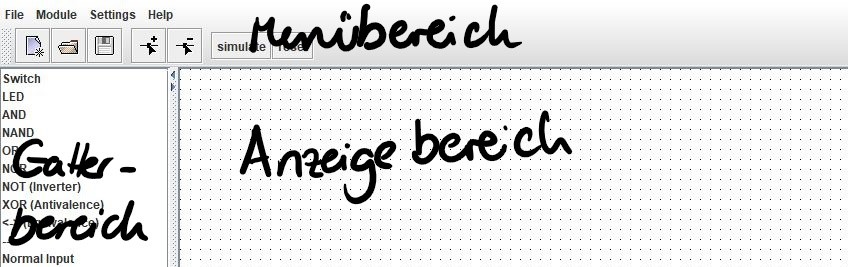
\includegraphics[width=0.55\textwidth]{../99_Bilder/LS.jpg}
		\end{wrapfigure}
		Oben links befindet sich der \textit{Menübereich}\(^*\), darunter teilt sich das Fenster ins den \textit{Gatterbereich}\(^*\) und den \textit{Anzeigebereich}\(^*\).\marginnote{\tiny{\(^*\) Die Bezeichnung sind selbst gewählt.}}\\
		Im oberen Bereich befinden sich die üblichen Menüfelder (\textit{File}, \textit{Module}, \textit{Settings} und \textit{Help}). Direkt darunter befinden sich Bild-Shortcuts zu den gängigsten Funktionalitäten (\textit{New}, \textit{Open} und \textit{Save}).\\
		\par\noindent
		\begin{wrapfigure}{l}{0.3\textwidth}
			\vspace{-10pt}
			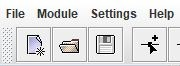
\includegraphics[width=0.35\textwidth]{../99_Bilder/menu_LS.jpg}
		\end{wrapfigure}
		Der shortcut \textit{\textbf{New}} erzeugt ein neues Dokument, in welchem eine Schaltungen unter Verwendung der zur Verfügung stehenden Gattern\(^{[1]}\)\marginnote{\textit{\tiny{\([1]\) logische Verknüpfung}}}.\\
		Mit dem shortcut \textit{\textbf{Open}} können zum einen gespeicherte Schaltungen aber auch gespeicherte Module\(^{[2]}\)\marginnote{\textit{\tiny{\([2]\)Gatter, das aus mehreren Gattern besteht - ähnlich zu einer Methode}}}[0.5cm]. Die geöffnete Datei wird in dem Anzeigebereich geöffnet und die Schaltung angezeigt.
		\subsection{Bestehende Module / Gatter nutzen}
		Um eine Schaltung zu realisieren, verwenden Sie die im Gatterbereiche angezeigten Gatter.
		\begin{wrapfigure}{r}{0.3\textwidth}
			\vspace{-10pt}
			\hspace{-15pt}
			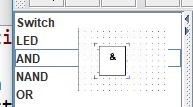
\includegraphics[width=0.35\textwidth]{../99_Bilder/gatter_LS.jpg}\\
		\end{wrapfigure}
		Um ein solches Gatter zu verwenden wählen Sie es aus 
		und führen die Maus in den Anzeigebereich. Dort wird ihnen das ausgewählte Gatter angezeigt und sie können es entsprechend positionieren.\\
		\par\noindent
		Nachfolgend finden Sie eine Auflistung der zur Verfügung stehenden Gatter (zunächst nur \textit{Switch, LED, AND, NAND, OR, NOR, NOT (Inverter), XOR (Antivalence)} und \textit{<-> (Equivalence)}\\
		\par\noindent
		\begin{tabularx}{\textwidth}{c|c|X}
			\textit{Bezeichnung} & \textit{Schaltungssymbol} & \textit{Erläuterung}\\
			\hline
			\hline
			Switch & 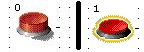
\includegraphics[width=0.1\textwidth, align=t]{../99_Bilder/switch.jpg} & Ist ein Input-Gatter. Entspricht einem Schalter mit den Zuständen 0 (OFF) und 1 (ON).\\
			\hline
			LED & 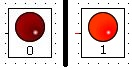
\includegraphics[width=0.1\textwidth,align=t]{../99_Bilder/LED.jpg} & Ist ein Output-Gatter. Die LED leuchtet, wenn sie ein Signal (1) erhält, ansonsten (0) ist sie aus.\\
			\hline
		\end{tabularx}
		\begin{tabularx}{\textwidth}{c|c|X|c}
			\textit{Bezeichnung} & \textit{Schaltungssymbol} & \textit{Erläuterung} & Wahrheitstabelle\\
			\hline
			\hline
			& & & \\
			\textbf{AND} & 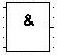
\includegraphics[width=0.1\textwidth, align=t]{../99_Bilder/AND.jpg} & Verknüpft die zwei Eingangssignale als ein logisches UND. Das Ausgangssignal ist \textbf{nur 1}, \underline{wenn beide} Eingangsvariabeln \textbf{1} sind. & \\
			\hline
			& & & \\
			\textbf{NAND} & 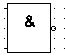
\includegraphics[width=0.1\textwidth,align=t]{../99_Bilder/NAND.jpg} & Die Verknüpfung entspricht dem AND. \textbf{Vorsicht:} Das Ausgangssignal wird invertiert. Also ist dieses \textbf{immer 1}, \underline{außer wenn beide} Eingangsvariablen \textbf{1} sind. & \\
			\hline
			& & & \\
			\textbf{OR} & 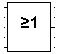
\includegraphics[width=0.1\textwidth, align=t]{../99_Bilder/OR.jpg} & Verknüpft die zwei Eingangssignale als ein logisches ODER. Das Ausgangssignal ist \textbf{1}, wenn \underline{eine} Eingangsvariable oder aber \underline{beide} Eingangsvariabeln \textbf{1} sind. & \\
			\hline
			& & & \\
			\textbf{NOR} & 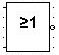
\includegraphics[width=0.1\textwidth,align=t]{../99_Bilder/NOR.jpg} & Die Verknüpfung entspricht dem OR. \textbf{Aber} das Ausgangssignal wird invertiert. Also ist dieses  \textbf{nur 1}, \underline{wenn beide} Eingangsvariablen \textbf{0} sind. & \\
			\hline
			& & & \\
			\textbf{NOT} & 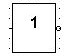
\includegraphics[width=0.1\textwidth, align=t]{../99_Bilder/NOT.jpg} & Dieses Gatter invertiert das Eingangssignal. Aus \textbf{0} wird \textbf{1} und umgekehrt (1 -> 0). & \\
			\hline
			& & & \\
			\textbf{XOR} & 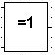
\includegraphics[width=0.1\textwidth,align=t]{../99_Bilder/XOR.jpg} & Die logische Verknüpfung OR wird hier verschärft. Das Ausgangssignal ist \textbf{nur genau dann 1}, \underline{wenn eine} der beiden Eingangssignale \textbf{1} ist. & \\
			\hline
			& & & \\
			\textbf{<->} & 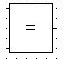
\includegraphics[width=0.1\textwidth, align=t]{../99_Bilder/equi.jpg} & Diese Verknüpfung ist das invertierte XOR. Also das Ausgangssignal ist \textbf{genau dann 1}, wenn \underline{beide} Eingangssignale \textbf{0} oder \textbf{1} sind. & \\
			\hline
		\end{tabularx}\\
		\par\bigskip\noindent
		\begin{wrapfigure}{l}{0.35\textwidth}
			\vspace{-20pt}
			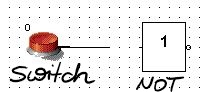
\includegraphics[width=0.4\textwidth]{../99_Bilder/connect.jpg}
		\end{wrapfigure}
		Möchten Sie zwei Gatter miteinander verbinden, so klicken sie auf den Ausgangspin des einen Gatters und ziehen die erscheinende Verbindungslinie auf den Eingangspin des anderen Gatters.\\
		\clearpage
		\par\noindent
		\begin{wrapfigure}{r}{0.3\textwidth}
			\hspace{-20pt}
			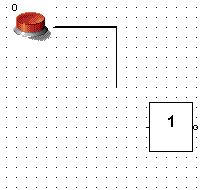
\includegraphics[width=0.35\textwidth]{../99_Bilder/connection.jpg}
		\end{wrapfigure}
		Aus Gründen der Übersichtlichkeit ist es zu empfehlen so häufig wie möglich gerade Verbindungen zu ziehen. Hierfür können Sie die zu ziehende Verbindungslinie aufbrechen. Dafür ziehen sie die Verbindung zu einem Punkt, betätigen die linke Maustaste und ziehen von diesem Punkt aus die nächste Verbindungslinie.\\
		LogicSim erzeugt, sobald sie eine Verbindungslinie starten, bei jedem Klick einen Zwischen-Verbindungspunkt.\\
		\subsection{Neue Module erstellen}
		Wie auch bei der Programmierung kommt es vor, dass gewünschte Funktionalitäten bzw. Gatter nicht zur Verfügung stehen. In einem solchen Fall haben Sie die Möglichkeit, ein eigenes Gatter zu erzeugen.\\
		\par\noindent
		\begin{wrapfigure}[8]{l}{0.25\textwidth}
			\vspace{-20pt}
			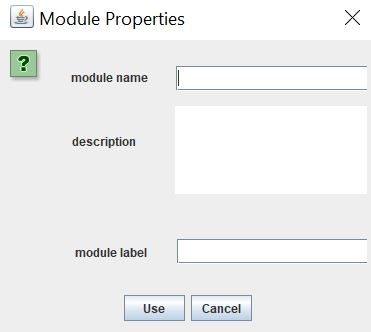
\includegraphics[width=0.3\textwidth,align=t]{../99_Bilder/new_mod.jpg}
		\end{wrapfigure}
		Hierfür wählen wir im Menüpunkt \textit{Modules -> Create Module} aus und geben einen \textit{module name} sowie ein \textit{module label}. Dabei wird der \textit{module name} im Gatterbereich angezeigt und das \textit{module label} wird auf dem Gatter angezeigt.\\
		\underline{Beispiel:} Das Gatter mit der Bezeichnung \textbf{AND} zeigt das Symbol \textbf{\&}.\\
		\par\bigskip\noindent
		\begin{wrapfigure}{r}{0.3\textwidth}
			\vspace{-10pt}
			\hspace{-25pt}
			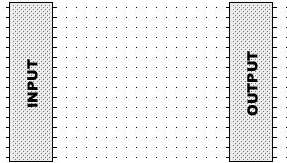
\includegraphics[width=0.35\textwidth]{../99_Bilder/inout.jpg}
		\end{wrapfigure}
		Haben Sie dies getan, erscheinen im Anzeigebereich ein Input-Gatter (16 Ein- und Ausgänge)  sowie ein Output-Gatter (16 Ein- und Ausgänge). Zwischen diesen beiden Gattern positionieren Sie die Gatter, die sie zur Realisierung ihres Moduls benötigen.\\
		Für ein funktionierendes Schaltmodul benötigen sie einen Input, welcher innerhalb des Moduls verarbeitet wird. Dieser Input kann aus einem aber auch aus bis zu 16 Eingangssignalen bestehen.\\
		Beachten Sie aber, dass sie die Eingänge von oben nach unten anbringen.\\
		Beachten Sie ebenso, dass das die Ein- und Ausgangspins auf einer Linie liegen. Bedeutet also, der erste Eingangspin geht auf den ersten Ausgangspin.\\
		\par\noindent
		\begin{wrapfigure}[7]{l}{0.3\textwidth}
			\vspace{-25pt}
			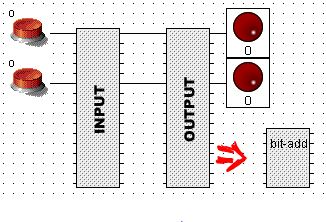
\includegraphics[width=0.35\textwidth]{../99_Bilder/falseInOut.jpg}
		\end{wrapfigure}
		\small{\textit{Bringen Sie beispielsweise ein Eingangssignal am ersten und am vierten Pin an, so wird ihr Gatter vier Gatter anbieten, obwohl nur zwei davon verwendet werden.\\
		Zudem weist ihr Modul dann auch vier Ausgänge aufweisen, da wie oben schon angedeutet, die Ein- und Ausgangspins in Reihe liegen.}}\\
		\par\noindent
		Haben Sie ihr Modul fertiggestellt, speichern Sie es. LogicSim speichert das Modul automatisch im Ordner \textit{LogicSim -> Modules}. Die Endung eines Moduls ist \textbf{\underline{.mod}}.
		\subsection{Module bearbeiten}
		\begin{wrapfigure}{l}{0.3\textwidth}
			\vspace{-10pt}
			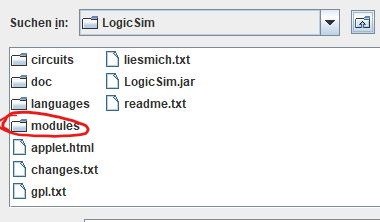
\includegraphics[width=0.35\textwidth]{../99_Bilder/folder_mod.jpg}
		\end{wrapfigure}
		Sie können bereits bestehende Module bearbeiten. Stellen Sie dafür sicher, dass ihr Anzeigebereich leer ist. Da der \textbf{open}-shortcut das Modul in ihren bereits vorhandenen Anzeigebereich öffnet.\\
		Am einfachsten ist es, wenn sie über den \textbf{New}-shortcut ein neues Dokument erzeugen. Im Anschluss betätigen Sie den \textbf{open}-shortcut. Es öffnet sich ein Auswahlfenster.\\
		Navigieren Sie in den Ordner \textit{LogicSim -> modules} und wählen Sie das zu bearbeitende Modul aus.
		\subsection{Schaltungen erzeugen und simulieren}
		\begin{wrapfigure}{r}{0.3\textwidth}
			\vspace{-10pt}
			\hspace{-25pt}
			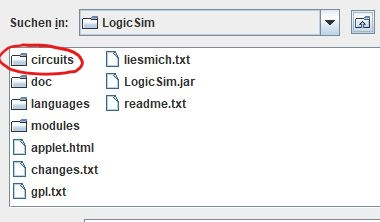
\includegraphics[width=0.35\textwidth]{../99_Bilder/folder_circ.jpg}
		\end{wrapfigure}
		Haben sie eine Schaltung erzeugt, sollten Sie diese zunächst speicher. Hierfür betätigen sie den \textbf{Save}-shortcut. Haben Sie die Schaltung bereits in einer Datei (Endung \textbf{.lsim}) gespeichert, wird diese überschrieben.\\
		
		\noindent
		Ansonsten öffnet sich ein Explorer-Fenster in welchem Sie den Ordner auswählen können, in dem Sie ihre Schaltung speichern wollen, zudem können Sie einen Dateinamen angeben.\\
		\par\noindent
		Um eine Schaltung zu testen, sie also zu simulieren, wählen Sie im Menübereich den shortcut \textbf{simulate}. LogicSim wechselt in den Simulierungsmodus. Es ist ihnen nun möglich Eingangssignale zu setzen. Dafür klicken Sie auf das entsprechende Gatter bzw. Modul.\\
		Verwendete Gatter hingegen werden blockiert, so dass sie diese nicht mehr verschieben können.\\
		\par\noindent
		\begin{tabularx}{\textwidth}{M|M}
			\textbf{Switch} & \textbf{binary Input} - zählt von 0 bis FF und konvertiert diese Zahl in 8 Bit (von oben nach unten)\\
			\hline
			\hline
			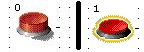
\includegraphics[width=0.45\textwidth,align=t]{../99_Bilder/switch.jpg} & 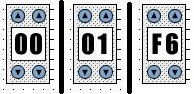
\includegraphics[width=0.45\textwidth,align=t]{../99_Bilder/binIn.jpg}
		\end{tabularx}
	\end{worksheet}
\end{document}